%\renewcommand{\lastmod}{April 29, 2020}

\chapter{Raman-Streuung}



%\begin{marginfigure}
%\inputtikz{\currfiledir rot_vib}
%\caption{Rotations-Vibrations-Übergänge liefert die P, Q, R-Zweige im Spektrum.}
%\end{marginfigure}
% 


\section{Ziele}

\begin{itemize}
\item Sie können die Raman-Streuung im Dipol-Modell und als inelastische Streuung an einem virtuellen Zustand erklären.

\item Sie können das Raman-Spektrum einfacher Moleküle wie das untenstehende erklären und daraus Eigenschaften der Rotation und Vibration sowie des Kernspins berechnen.

\end{itemize}

\begin{figure}
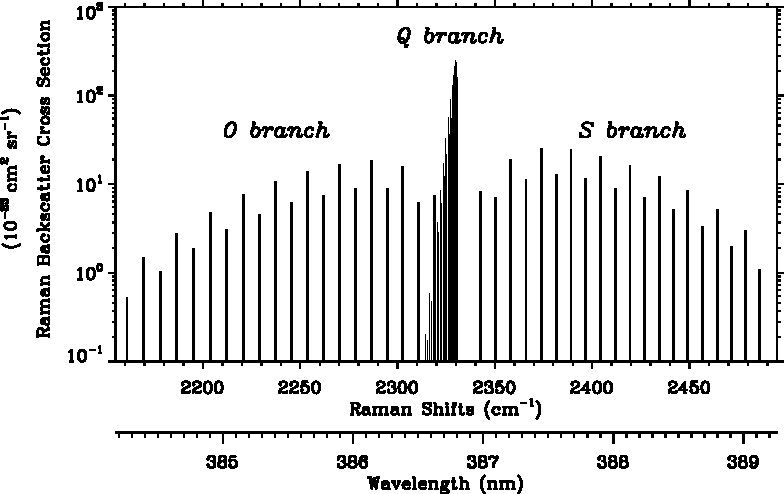
\includegraphics[width=\textwidth]{\currfiledir oe/OE_n2_fig1.pdf}
\caption{Raman-Spektrum von \ch{N2} in der Atmosphäre gemessen mit einem Laser der Wellenlänge 354.8~nm. Darstellung leicht modifiziert aus \cite{Liu14_OE_N2}. }
\end{figure}


\section{Wie misst man das?}

Moleküle ohne permanentes Dipolmoment (also beispielsweise homonukleare Moleküle) zeigen im THz-Absorptionsspektrum kein Rotationsspektrum. Moleküle ohne  Variation des Dipol-Moments mit der Normal-Koordinate zeigen kein Vibrationsspektrum im Infraroten. Solche
Moleküle sind trotzdem spektroskopierbar, nämlich über den Raman-Effekt.

Der Raman-Effekt\sidenote{nach Chandrasekhara Venkata Raman, 1888--1970} ist die \emph{inelastische} Streuung von Licht an Materie, bei der sich also die Frequenz des Lichts ändert. Dies ist im Gegensatz zur Rayleigh-Streuung, die die \emph{elastische} Streuung von Licht beschreibt. Nur wenige Photonen werden inelastisch gestreut. Der Effekt ist daher mit dem Auge nicht wahrzunehmen und man benötigt eine spektral schmale und intensive Lichtquelle, also einen Laser. Diesen scheint man auf bzw. durch die Probe.\sidenote{Wir diskutiere hier Raman-Spektroskopie an Gasen. Raman-Streuung an festen Proben wird aber ebenfalls sehr oft zur Charakterisierung von Materialien eingesetzt.} Im Gegensatz zu den Spektroskopie-Methoden, die wir bisher betrachtete haben, wird hier das Licht \emph{senkrecht zur Stahlrichtung} detektiert. So misst man nur gestreutes Licht, nicht direkt den Laser. In einem hochauflösenden Spektrometer findet man dann bei drei Frequenzbereichen Photonen
\begin{itemize} \setlength{\itemsep}{0pt}
\item bei der Laser-Frequenz $\bar{\nu}_\text{laser}$. Dies ist die elastische Rayleigh-Streuung.
\item bei $\bar{\nu} < \bar{\nu}_\text{laser}$ inelastisch unter Energieverlust  gestreutes Licht. Dies nennt man Stokes-Linie. Sie ist etwa $10^{5}$ mal schwächer als die Rayleigh-Linie.
\item bei $\bar{\nu} > \bar{\nu}_\text{laser}$ inelastisch unter Energiegewinn gestreutes Licht. Dies nennt man Anti-Stokes-Linie. Sie ist noch einmal $10$ bis $100$ mal schwächer als die Stokes-Linie.
\end{itemize}
Die hier als Stokes- bzw. Anti-Stokes-Linie bezeichneten 'Linien' besitzen eine deutliche Struktur, sehr analog zu den Rotations-Vibrations-Spektren und beinhalten die gleiche Information über das Molekül.


\section{Klassische Erklärung des Schwingungs-Raman-Effekts}

Wir beginnen mit einer klassischen, makroskopischen Erklärung des Raman-Effekts. Das Molekül habe kein permanentes Dipolmoment, sei aber polarisierbar mit der Polarisierbarkeit $\alpha$. Zunächst vernachlässigen wir auch Rotation und Vibration des Moleküls. Dann ist das induzierte Dipolmoment
\begin{equation}
p_\text{ind}(t) = \alpha E(t) = \alpha E_0 \cos \omega_0 t
\end{equation}
Das Dipolmoment oszilliert also mit der Lichtfrequenz $\omega_0$. Laut den Maxwell-Gleichungen strahlen bewegte Ladungen elektromagnetische Felder ab, so auch dieses oszillierende Dipolmoment. Dies ist die Rayleigh-Streuung. Genauere Rechnungen zeigen, dass die Intensität proportional zu $\omega^4$ ist. Der Himmel ist also blau, weil blaues Licht besser Rayleigh-Streuung macht.

Nun erlauben wir die Vibration des Moleküls. Die Polarisierbarkeit hängt dann, bei passenden Molekülen, vom Kern--Kern--Abstand $R$ ab. Dies nähern wie in einer Taylor-Reihe
\begin{equation}
\alpha = \alpha(R) = \alpha(R_0) + \left. \frac{\partial \alpha}{\partial R} \right|_{R_0}  \left( R - R_0 \right) + \dots
\end{equation}
Der Kern--Kern--Abstand $R$ ändert sich periodisch mit der Schwingungs-Frequenz $\omega_\text{vib}$ und der Amplitude $q$, also
\begin{equation}
\left( R - R_0 \right) = q \, \cos \omega_\text{vib} t
\end{equation}
Nun berechnen wir analog zu oben das induzierte Dipolmoment
\begin{align}
p_\text{ind}(t) = & \alpha(t) E(t) \\
= & \alpha(R_0) E_0 \cos(\omega_0 t) +
\left. \frac{\partial \alpha}{\partial R} \right|_{R_0}   q \,  E_0 \, \cos (\omega_\text{vib} t)  \cos(\omega_0 t) \\
= & \underbrace{  \alpha(R_0) E_0 \cos(\omega_0 t) }_\text{Rayleigh} \\
& + \left. \frac{\partial \alpha}{\partial R} \right|_{R_0}  \frac{ q \,  E_0 }{2} 
\Bigl\{ 
\underbrace{ \cos \left( [\omega_0 -\omega_\text{vib}] t \right)}_\text{Stokes}  +  \underbrace{\cos \left( [\omega_0 + \omega_\text{vib}] t \right)  
}_\text{Anti-Stokes} 
\Bigr\} 
\nonumber
\end{align}
Das durch das oszillierende Dipolmoment abgestrahlte elektromagnetische Feld liefert wieder die Rayleigh-, jetzt aber auch die Stoks- und Anti-Stokes-Linie.

Allgemein gilt, auch nach 'moderner' Rechnung, dass Schwingungsmoden dann Raman-aktiv sind, wenn die  Polarisierbarkeit von $R$ abhängt, also 
\begin{equation}
\left. \frac{\partial \alpha}{\partial R} \right|_{R_0} \neq 0
\end{equation}
Dies ist in zweiatomigen Molekülen \emph{immer} der Fall. In mehr-atomigen Molekülen \emph{mit Inversionssymmetrie} sind Raman-Aktivität und IR-Aktivität komplementär. Ein Beispiel dazu ist \ch{CO2}. Die symmetrische Streckschwingung ist nicht Infrarot-aktiv, aber im Raman-Spektrum sichtbar. Die asymmetrische Streckschwingung verhält sich genau umgekehrt.


\section{Mikroskopische Überlegungen}

Beim Raman-Prozess wechselwirken zwei Photonen mit dem Molekül, das einfallende und das auslaufende. Die quantenmechanische Beschreibung benötigt deshalb eine Störungstheorie zweiter Ordnung. Dies geht hier zu weit, ist aber beispielsweise in Kapitel 17 von \cite{Haken_wolf_II} dargestellt. Hier betrachten wir nur qualitative Argumente, die zumindest das Amplitudenverhältnis zwischen Stokes und Anti-Stokes-Linie erklären können. Diese sind nach obigen klassischen Überlegungen ja noch gleich stark.

Atome und Moleküle haben in der Quantenmechanik diskrete Energieniveaus. Photonen passender Frequenz können dann absorbiert werden. In der schematischen Darstellung verbindet ein senkrechter Pfeil zwei Niveaus.

\begin{marginfigure}
\begin{tikzpicture}
\begin{scope}
\draw[line width=1pt] (0,0) -- (1,0);
\draw[line width=1pt] (0,2) -- (1,2);
\draw[->] (0.5,0) -- (0.5,2);
\end{scope}
\begin{scope}[xshift=2cm]
\draw[line width=1pt] (0,0) -- (1,0);
\draw[line width=1pt, dashed] (0,2) -- (1,2);
\draw[->] (0.5,0) -- (0.5,2);
\end{scope}
\end{tikzpicture}
%\caption{Rotations-Vibrations-Übergänge liefert die P, Q, R-Zweige im Spektrum.}
\end{marginfigure}
 

Was passiert mit Photonen unpassender Frequenz? Diese können nicht absorbiert werden, dies würde schließlich die Energieerhaltung verletzten, aber sie werden gestreut. In der schematischen Darstellung zeichnet man dazu einen virtuellen Zustand als strichlierte horizontale Linie an das Ende des 'Photon'-Pfeils. Virtuelle Zustände können nicht bevölkert werden. Es gibt sie ja nicht wirklich. Auf der anderen Seite gibt es die Energie--Zeit--Unschärfe
\begin{equation}
\Delta E \cdot \Delta t \ge \hbar
\end{equation}
Wenn die Zeitdauer $\Delta t $ nur klein genug ist, dann muss die Energie-Unschärfe $\Delta E $ sehr groß werden. Für sehr kurze Zeiten kann man sozusagen gar nicht wissen, ob das Photon die passende Energie hat. Das kann man quantenmechanisch korrekt mit der Dichtmatrix formulieren. Für uns reicht hier, dass auch 'unpassende' Photonen mit diskreten Niveaus in Atomen oder Molekülen wechselwirken können, wenn auch nur für sehr kurze Zeit, wenige Femtosekunden für sichtbares Licht.

\begin{marginfigure}
\inputtikz{\currfiledir lorentz_oszillator}
\caption{Der dispersive Anteil des Lorentz-Oszillators fällt langsamer ab als der absorptive. }
\end{marginfigure}
 

Ein zweiter Gesichtspunkt kommt vom Lorentz-Oszillator aus Kapitel \ref{chap:3_diel}. Wir können diskrete atomare Übergänge als Lorentz-Oszillator beschreiben. Die Absorptionslinie hat das eben die bekannte Lorentz-Form. Sie fällt sehr schnell ab, wenn $| \omega  - \omega_0 |$ groß wird. Der Oszillator hat aber auch einen dispersiven Anteil, der den Realteil des Brechungsindexes beschreibt. Dieser fällt viel langsamer ab als der absorptive. Fern von der Resonanz ist er also wichtiger. Wir können uns ein Atom / Molekül fern von der Resonanz als als kleines Volumen mit einen etwas von Vakuum verschiedene Brechungsindex vorstellen, das aber nicht absorbiert. Solch eine Brechungsindex-Variation führt aber zu Streuung von Licht.

\begin{marginfigure}%[-50mm]
\inputtikz{\currfiledir fig_raman_states}
\caption{Stokes- und Anti-Stokes-Streuung über einen virtuellen Zustand (strichliert). Die spektrale Position de Rayleigh-Linie entspricht der des einfallenden Lasers.}
\end{marginfigure}
 

Nach diesen Vorüberlegungen können wir das Zustandsdiagramm für den Raman-Effekt zeichnen, wenn das Molekül mehrere äquidistante Schwingungszustände hat, die mit der Quantenzahl $\nu$ durchnummeriert sind. Der Abstand der Schwingungszustände $\hbar \omega_\text{vib}$ ist klein gegen die Energie des Photons $\hbar \omega_0$. Das Photon wird an einem virtuellen Zustand gestreut. Das dabei entstehende zweite Photon wird abgestrahlt und durch den Pfeil nach unten symbolisiert. Dieser Pfeil kann entweder auf den Ausgangszustand $\nu = 0$ zurück gehen. Das ist Rayleigh-Streuung. Oder er endet auf einem höheren Zustand und liefert die Stokes-Linien bei niedrigerer Energie. Die Anti-Stokes-Linien erhält man, wenn man nicht von $\nu = 0$ ausgeht, sondern von einem höheren Zustand, und dann aber bis auf $\nu = 0$ zurück fällt. Damit ist die Energie des auslaufenden Photons größer als die des einfallenden.



Damit lassen sich verschiedene Aspekte des Raman-Effekts erklären: er ist sehr schwach, weil zwei Photonen quasi gleichzeitig ($\Delta t \approx 1$~fs) wechselwirken müssen. Die Intensität der Linien ist proportional zur Besetzung der Ausgangs-Schwingungszustände, also entsprechend einem Boltzmann-Faktor
\begin{equation}
\frac{I_\text{anti-Stokes}}{I_\text{Stokes}} = 
\frac{N_{\nu = 1}}{N_{\nu = 0}} =
 e^{- \frac{\hbar \omega_\text{vib}}{k_b T}}
\end{equation}
Bei Vibrationsfrequenzen von etwa $1000$~cm$^{-1}$ und $k_B T \approx 200 $~cm$^{-1}$ bei Raumtemperatur ist das Intensitätsverhältnis also $e^{-5} \approx 1 /150$. Man kann das Verhältnis der Linien also als lokales Thermometer benutzen.

Die quantenmechanischen Rechnungen ergeben die selben Auswahlregeln wie für die Infrarot-Schwingungsspektroskopie, also 
\begin{equation}
 \Delta \nu = \pm 1 \quad \text{falls harmonisch, sonst} \quad \pm 1, \pm 2, \dots  
\end{equation}



\section{Der Rotations-Raman-Effekt}

Ähnlich zu molekularen Schwingungen findet sich auch die Rotation der Moleküle im Raman-Spektrum. Wir beginnen wieder mit dem klassischen Modell. Elektromagnetisches Feld $E(t)$ und induziertes Dipolmoment $p_\text{ind}(t)$ sind wie oben
\begin{equation}
p_\text{ind}(t) = \alpha(t) E(t) = \alpha(t) E_0 \cos \omega_0 t \label{eq:raman_pind_rot}
\end{equation}
In die Zeitabhängigkeit der Polarisierbarkeit $\alpha(t)$ bauen wir jetzt die Rotation ein. Dazu nehmen wir an, dass die Polarisierbarkeit anisotrop ist, sich also für zwei senkrecht aufeinander stehende Richtungen unterscheidet: $\alpha_\parallel \neq \alpha_\perp$. Bei einem sich mit der Kreisfrequenz $\omega_R$ drehenden Molekül ist die Polarisierbarkeit also
\begin{equation}
\alpha(t) = \alpha_0 + \Delta \alpha \cos ( 2 \omega_R t) \quad \text{mit} \quad \Delta \alpha = \alpha_\parallel - \alpha_\perp
\end{equation}
Der Faktor $2$ kommt daher, dass das Molekül bereits nach $180^\circ$ wieder in sich übergeht. Dies setzen wir wieder in Gl. \ref{eq:raman_pind_rot} ein und multiplizieren aus. Wir bekommen analog zu oben
\begin{align}
p_\text{ind}(t) = & \underbrace{  \alpha_0 E_0 \cos(\omega_0 t) }_\text{Rayleigh} \\
& +   \frac{ \Delta \alpha \,  E_0 }{2} 
\Bigl\{ 
\underbrace{ \cos \left( [\omega_0 -2 \omega_R] t \right)}_\text{Stokes}  +  \underbrace{\cos \left( [\omega_0 + 2 \omega_R] t \right)  
}_\text{Anti-Stokes} 
\Bigr\} 
\nonumber
\end{align}
Die Linien sind also bei der doppelten Rotationsfrequenz ober- oder unterhalb der Rayleigh-Linie. Quantenmechanische Rechnungen ergeben als Auswahlregeln entweder
\begin{equation}
\Delta J = 0 \quad \text{und falls} \quad  \Delta \alpha \neq 0 \quad  \text{dann auch} \quad \Delta J = \pm 2
\end{equation}
Die Position der Linien in einem Rotations-Raman-Spektrum sind also
\begin{equation}
 \bar{\nu} =  \bar{\nu}_\text{laser} \pm B \left[ (J+2) (J+3) - J(J+1) \right] = 
 \bar{\nu}_\text{laser} \pm B \left[ 4J + 6 \right]
\end{equation}
wobei das $+$ die Anti-Stokes-Banden und das $-$ die Stokes-Banden liefert. Der Abstand der äquidistanten Linien ist damit nicht mehr $2B$ wie im Fall des THz-Absorptions-Spektrums, sondern $4B$. Da $B$ klein gegenüber $\bar{\nu}_\text{laser} $ ist, ist ein reines Rotations-Raman-Spektrum messtechnisch aufwändig. Eine sehr schwache Linie muss in kleinem spektralen Abstand zur starken Rayleigh-Linie detektiert werden. Dies erfordert einen hochauflösenden und stark unterdrückenden Monochromator, quasi immer durch die Hintereinanderschaltung von zwei oder drei Monochromatoren zu einem Doppel- bzw. Trippel-Monochromator realisiert.




\begin{marginfigure}
\inputtikz{\currfiledir rot_vib_raman}
\caption{Rotations-Vibrations-Spektrum in Raman-Streuung. Alle gezeichneten Linien und Übergänge sind Stokes-Übergänge. Die Rayleigh-Linie liegt rechts außerhalb des Bildes, das entsprechende Anti-Stokes-Spektrum noch höherenergetischer. \label{fig:raman_rotvib}}
\end{marginfigure}

 \section{Rotations-Vibrations-Raman-Effekt}

Analog zum Rotations-Vibrations-Spektrum in Absorption lässt sich die kombinierte Anregung eines Rotations- und Schwingungsniveaus auch im Raman-Effekt beobachten. Abbildung \ref{fig:raman_rotvib} skizziert die beteiligten Zustände für die Stokes-Bande, also die Linien die niederenergetisch von der Rayleigh-Linie liegen. Die Linienpositionen sind 

\begin{equation}
 \bar{\nu} =  \bar{\nu}_\text{laser} \pm \bar{\nu}_\text{vib} \pm B \left[ 4J + 6 \right]
\end{equation}
Das erste $\pm$ unterscheidet zwischen Stokes ($-$) und Anti-Stokes ($+$). Das zweite $\pm$ entsprechend dem Vorzeichen von $\Delta J$. Man beachte, dass die Sequenz von äquidistanten Rotations-Linien wieder mit dem Abstand $6B$ von der reinen Vibrationslinie  $\Delta J = 0$ beginnt. Ähnlich zum Absorptionsspektrum werden die Linien mit $\Delta J =-2$ als O-Zweig, die mit 
$\Delta J =+2$ als S-Zweig bezeichnet.



\begin{margintable}
\begin{tabular}{rccccc}
$\Delta J$ & -2 & -1 & 0 & 1 & 2 \\
Zweig & O & P & Q & R & S
\end{tabular}
\caption{Nomenklatur der Zweige bei Rotationsspektren. $\Delta J = \pm 1$ im Absorptionsspektrum, $\Delta J = \pm 2$ im Raman-Spektrum sichtbar.}
\end{margintable}

\section{Einfluss der Kernspins}

Man beobachtet, dass das Rotations-Raman-Spektrum von zweiatomigen Molekülen aus zwei identischen Atomen eine charakteristische Intensitätsmodulation der Linien zeigt. Die Abbildung am Anfang des Kapitels ist ein Beispiel. Die Ursache dafür ist der Kernspin.

\begin{margintable}

\begin{tabular}{cc}
Molekül & $J_\text{ungerade}$  : $J_\text{gerade}$  \\ \hline
\ch{^1H2} & 3:1 \\
\ch{^2H2} & 1:2 \\
\ch{^{14}N2} & 1:2 \\
\ch{^{16}O2} & 1:0 
\end{tabular}
\caption{Beispiele für beobachtete Amplitudenverhältnisse.}
\end{margintable}


Atomkerne sind entweder Fermionen, haben also einen halbzahligen Spin, oder sie sind Bosonen, haben also einen ganzzahligen Spin. Für Fermionen muss die Gesamt-Wellenfunktion anti-symmetrisch unter Vertauschung sein, für Bosonen symmetrisch. Die Frage ist also, wie sich die einzelnen Komponenten der Wellenfunktion ändern, wenn wir die beiden Atomkerne im Molekül vertauschen.
 
Die \emph{Kernwellenfunktion} kann entweder die symmetrische oder die anti-symmetrische Kombination der beiden (identischen) Kernspins sein.
Die \emph{Elektronenwellenfunktion} ist gegenüber der Vertauschung der Kerne, also effektiv der Inversion der Koordinaten, fast immer symmetrisch. Prominente Ausnahme ist \ch{O2}, das einen Triplett-Grundzustand $^3\Sigma_g^-$ hat, wie wir bei der Diskussion der Termsymbole in Kapitel 3 gesehen haben. Die \emph{Vibrations-Wellenfunktion} ist immer symmetrisch gegen Vertauschung der Kerne. Die \emph{Rotations-Wellenfunktion} in zweiatomigen Molekülen ist anti-symmetrisch für ungerade Quantenzahlen $J$, also $J = 1,3, 5, \dots$ und symmetrisch für gerade $J$.


Die Symmetrie der Gesamt-Wellenfunktion ist das Produkt der einzelnen Symmetrien. Für fermionische Kerne muss die Gesamt-Funktion anti-symmetrisch sein, für bosonische Kerne symmetrisch. Damit beeinflusst die Symmetrie der Kern-Wellenfunktion die 'Geradheit' der Rotationsquantenzahl $J$. Und die statistischen Gewichte der beiden Symmetrien der Kern-Wellenfunktion ist unterschiedlich. Für Kerne mit $I = 1/2$ gibt es eine anti-symmetrische Kombination (analog dem Singulett für Elektronen) und drei symmetrische Kombinationen (analog dem Triplett für Elektronen). Allgemein ist das Verhältnis der statischen Gewichte $g$
\begin{equation}
 \frac{g_\text{symmetrisch}}{g_\text{anti-symmetrisch}} = \frac{I + 1}{I}
\end{equation}
Für fermionische Kerne ($I$ halbzahlig) ist damit 
\begin{equation}
 \frac{g(J = \text{ungerade}) }{g(J = \text{gerade})} = \frac{I + 1}{I}
\end{equation}
und für bosonische Kerne ($I$ ganzzahlig) gerade anders herum
\begin{equation}
 \frac{g(J = \text{ungerade}) }{g(J = \text{gerade})} = \frac{I}{I +1}
\end{equation}
Und wenn die elektronische Wellenfunktion  doch anti-symmetrisch sein sollte (Sauerstoff!), dann eben gerade andersherum.

\paragraph{Beispiel \ch{^1H2}} Jeder Kern hat $I = 1/2$, ist also ein Fermion und die Gesamt-Wellenfunktion muss anti-symmetrisch unter Vertauschen der beiden Kerne sein. Die Vibrations-Wellenfunktion und der elektronische Grundzustand sind symmetrisch, fallen bei der Multiplikation der Gesamt-Wellenfunktion also nicht ins Gewicht. Die Kern-Wellenfunktion kann sein
\begin{itemize}
\item \emph{anti-symmetrisch}, also $M_I = 0$. Damit die Symmetrie insgesamt anti-symmetrisch bleibt, muss der Rotationsanteil symmetrisch sein, also $J = \text{gerade}$. Dies nennt man \emph{para-Wasserstoff} und hat das statische Gewicht 1.

\item \emph{symmetrisch}, also $M_I = 0, \pm 1$. Damit die Symmetrie insgesamt anti-symmetrisch wird, muss der Rotationsanteil anti-symmetrisch sein, also $J = \text{ungerade}$. Dies nennt man \emph{ortho-Wasserstoff} und hat das statische Gewicht 3.
\end{itemize}
%
Da die Auswahlregeln $\Delta J = 2$ bei Raman-Übergängen verlangen, sind Übergänge ohne Änderung des Spins in einem Sub-System möglich. Es gibt im Wasserstoff-Molekül \ch{^1H2} also zwei Sätze von Linien, gerade und ungerade $J$, wobei die ungeraden um den Faktor 3 intensiver sind.




\paragraph{Beispiel \ch{^{16}O2}} Jeder Kern hat $I = 0$, ist also ein Boson und die Gesamt-Wellenfunktion muss symmetrisch unter Vertauschen der beiden Kerne sein. Die Vibrations-Wellenfunktion ist symmetrisch. Der elektronische Grundzustand $^3\Sigma_g^-$ ist allerdings eine Ausnahme, ein Triplett und damit anti-symmetrisch. Bei verschwindendem Spin $I=0$  der einzelnen Kerne ist die Summe der Kernspins immer Null. Damit gibt es nur eine Kern-Wellenfunktion und die ist symmetrisch. Damit die Gesamt-Wellenfunktion symmetrisch bleibt, muss die Rotations-Wellenfunktion anti-symmetrisch sein, also $J = \text{ungerade}$. In Sauerstoff-Molekül  \ch{^{16}O2} fehlen also die Rotationslinien mit geradem $J$ vollständig. Wenn man den Kernspin nicht berücksichtigen würde, dann würde man eine doppelt so große Rotationskonstante $B$ annehmen.





\printbibliography[segment=\therefsegment,heading=subbibliography]
